\section{Weiterführende Arbeiten}
\subsection{Entwicklung einer Zähleinrichtung}
Der in dieser Arbeit entwickelte Prototyp ist darauf ausgelegt, zuvor durchgeführte
Wireshark-Messungen auszuwerten.
Damit Messungen in der Praxis, beispielsweise in einem Zug oder Tram durchgeführt
werden können, muss der Prototyp dahingehend erweitert werden, dass 
Probe-Requests kontinuierlich erfasst und ausgewertet werden können.
Dazu wurden ein Architekturvorschlag erarbeitet, der in einer künftigen 
Arbeit als Anhaltspunkt dienen kann.

\subsubsection*{Architekturvorschlag}
Eine Möglichkeit, wie die Architektur einer Zähleinrichtung aufgebaut werden könnte,
wird in der Abbildung~\ref{figure:architectureproposal} dargestellt.

\begin{figure}[h!]
    \centering
    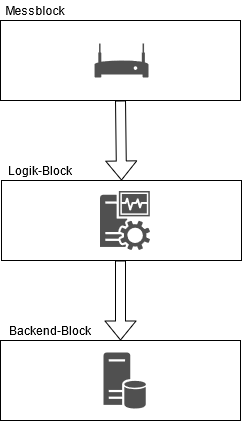
\includegraphics[width=0.5\linewidth]{architectureproposal.png}
    \caption{Architekturvorschlag für eine Zähleinrichtung}
    \label{figure:architectureproposal}
\end{figure}

\clearpage

Im Messblock befinden sich ein oder mehrere Access-Points oder Messantennen, 
welche ankommende Probe-Requests erfassen und an den Logik-Block weiterleiten.
Der Logik-Block ist für die Sortierung und Filterung der ankommenden Probe-Requests
verantwortlich. Die Resultate werden dann an einen Backend-Block weitergeleitet,
welcher für eine Persistierung der Ergebnisse und allfällige Auswertungen 
verantwortlich ist. Falls die Architektur mit einem IOT-Ansatz umgesetzt wird, 
kann durch eine Vorfilterung im Messblock die benötigte Bandbreite für die 
Übertragung reduziert werden. Weiterhin muss in solch einem Ansatz evaluiert 
werden, ob sich der Logik-Block vor Ort in Form eines Gateway befindet oder 
auf dem Server realisiert wird.

Ein weiterer möglicher Ansatz für eine Zähleinrichtung ist die Verwendung 
von Raspberry Pi als abgeschlossenes Zählsystem. Es ist möglich mit einem -
oder mehreren - Raspberry Pi mit WLAN-Dongles ein Messsystem zu entwickeln, 
welches Probe-Requests erfassen und filtern kann. Eine Möglichkeit ist 
die Verwendung eines der Python-Module 
"Pyshark" \footnote{Dokumentation: \url{https://kiminewt.github.io/pyshark/}}
oder "Scapy" \footnote{Dokumentation: \url{https://scapy.readthedocs.io/en/latest/introduction.html}} 
welche beide in der lage sind, WLAN-Daten zu erfassen und zu filtern.


\subsection{Erweiterung der Filterung - Algorithmen}
Eine zusätzliche Möglichkeit, den Prototypen zu verbessern, ist, die 
Algorithmen zu erweitern. Die Filterregeln können beispielsweise durch 
Machine-Learning-Algorithmen dahingehend angepasst werden, dass der 
Prototyp selbständig und kontinuierlich die Klassifikation der Probe-Requests 
ver-bessert.

Dazu müssten weitere Messungen durchgeführt werden, in denen mehrere Geräte 
zur selben Zeit mit verschiedenen Einstellungen in Betrieb sind. 
Dieses Vorgehen würde einen Supervised-Learning-Ansatz ermöglichen.
Alternativ kann auch mit Datensets aus der Praxis gearbeitet werden, 
welche mit einem Unsupervised-Learning-Ansatz einen Algorithmus trainieren.

Werden mehrere Messantennen für die Aufzeichung von Probe-Requests verwendet,
können zusätzliche Informationen bei den Messdaten hinzukommen. 
Beispielsweise ist die Information, welche Antenne den Probe-Request aufgezeichnet
hat, in einer Filterung verwendbar. Allerdings muss darauf geachtet werden, 
dass Frames von einem Gerät, die von mehreren Antennen gleichzeitig aufgezeichnet 
werden, nicht als separate Frames interpretiert werden.

\subsection{Erweiterung der Filterung - Messungen}
In dieser Arbeit wurden zwölf verschiedene Geräte mit insgesamt dreizehn 
Betriebssystemversionen getestet. Die neuste Android-Version 11 konnte nur
auf einem Gerät getestet werden, da die gerätespezifische Android-11-Version 
auf keinem der getesteten Geräte zur Verfügung stand. Weitere Messungen auf 
diesen Gerätetypen mit der Android Version 11 können neue Erkenntnisse 
generieren, mit denen der Prototyp weiter verbessert werden kann oder 
die eine Unterscheidung von Geräten komplett unmöglich machen.

Weiterhin können andere moderne Geräte getestet werden, um den Katalog von 
Geräteverhalten zu erweitern und den Prototypen zu verbessern.

\subsection{Erweiterung der Aufzeichnungsmethoden}
Im Rahmen dieser Arbeit wurde das Verhalten der Mobilgeräte beim Aus-senden 
von Probe-Requests erfasst. Künftige Arbeiten könnten neben Probe-Requests auch 
weitere Informationen von Mobilgeräten aufzeichnen. Eine mögliche Informationsquelle
wären Bluetooth-Signale oder andere Frame-Typen aus der Sicherungsschicht.

Zudem gibt es im Forschungsfeld der Indoor-Lokalisierung den Ansatz, die 
Position eines Mobilgeräts anhand der Signalstärke zu triangulieren.

\clearpage